\section{Ứng dụng thực tế}
\subsection{Market Basket Analysis — Thien}
\label{sec:basket}
Phân tích giỏ hàng (market basket analysis) tìm các nhóm sản phẩm thường được mua
cùng nhau để nhà bán lẻ sắp xếp, đóng gói hoặc khuyến mãi. Nhóm dùng bộ dữ liệu
Online Retail II~\cite{chen2012}, giấy phép CC BY 4.0, gồm mọi dòng hóa đơn của
một cửa hàng quà tặng trực tuyến tại Anh từ 01/12/2009 đến 09/12/2011. Tệp CSV
được tải từ hai bản sao trên Hugging Face, cố định theo revision; hai bản giống
nhau từng byte và có đúng 1\,067\,371 dòng như UCI công bố. Mã băm SHA-256 của
tệp được kiểm tra trước khi xử lý.

Mỗi giao dịch (transaction) là một hóa đơn (invoice), và mỗi item là một mã sản
phẩm (stock code) viết hoa, vì \texttt{85123a} và \texttt{85123A} chỉ cùng một
sản phẩm. Mã số nguyên của item được gán theo thứ tự mã sản phẩm bằng hàm
\texttt{encode\_transactions}, nên ánh xạ không phụ thuộc thứ tự dòng và đảo ngược
được: tệp \texttt{items.tsv} lưu mã số, mã sản phẩm, mô tả thường gặp nhất và số
giỏ hàng chứa sản phẩm. Bảng~\ref{tab:basket-cleaning} cho thấy tác động của từng
bước làm sạch.

\begin{table}[t]
\centering
\caption{Số dòng và số hóa đơn sau từng bước làm sạch Online Retail II}
\label{tab:basket-cleaning}
\begin{tabular}{lrrr}
\hline
Bước & Bỏ & Còn (dòng) & Hóa đơn \\
\hline
Dữ liệu gốc & & 1\,067\,371 & 53\,628 \\
Dòng trùng lặp & 34\,335 & 1\,033\,036 & 53\,628 \\
Hóa đơn hủy (C) & 19\,104 & 1\,013\,932 & 45\,336 \\
Điều chỉnh nợ xấu (A) & 6 & 1\,013\,926 & 45\,330 \\
Số lượng $\le 0$ & 3\,393 & 1\,010\,533 & 41\,937 \\
Đơn giá $\le 0$ & 2\,621 & 1\,007\,912 & 40\,076 \\
Mã không phải sản phẩm & 4\,555 & 1\,003\,357 & 39\,516 \\
\hline
\end{tabular}
\end{table}

UCI công bố dữ liệu thành hai sheet theo năm, và cả hai đều chứa các ngày 1--9
tháng 12 năm 2010, chiếm 22\,844 trong số 34\,335 dòng trùng. Dòng trùng không làm
thay đổi giỏ hàng vì item lặp lại trong một giao dịch được gộp. Hóa đơn hủy là
hóa đơn riêng mang tiền tố C dùng để đảo một giao dịch bán trước đó, nên bỏ nó
giữ nguyên giỏ hàng khách đã mua. Các dòng có số lượng hoặc đơn giá không dương là
ghi chú kho như ``check'' hay ``damaged'', không phải giao dịch bán; hai bước này
bỏ 5\,254 hóa đơn chỉ gồm ghi chú và 380 mã chưa từng được bán. Bước cuối bỏ các
mã dịch vụ như phí vận chuyển, giảm giá, phí ngân hàng và phiếu quà tặng; riêng
phí vận chuyển xuất hiện trong 8,8\% số hóa đơn nên sẽ tạo luật giả với mọi sản
phẩm phổ biến. Dòng không có mã khách hàng vẫn được giữ vì một hóa đơn là một giỏ
hàng bất kể ai trả tiền.

Kết quả gồm 39\,516 giỏ hàng trên 4\,725 sản phẩm. Độ dài giỏ hàng có trung vị
15, phân vị 90 là 51, trung bình 25,1 và lớn nhất 1\,106 ở các đơn bán sỉ; 92\%
số giỏ hàng đến từ Anh. Với Eclat của nhóm, minsup 0,01 (396 hóa đơn) cho
1\,355 tập phổ biến, trong đó 648 tập có từ hai sản phẩm trở lên.

\subsubsection{Luật kết hợp}
Một luật kết hợp (association rule) $X \Rightarrow Y$ gồm vế trái (antecedent)
$X$ và vế phải (consequent) $Y$ là hai tập sản phẩm khác rỗng, rời nhau. Gọi
$N$ là số giỏ hàng và $\sigma(Z)$ là số giỏ hàng chứa mọi sản phẩm của tập $Z$.
Ba độ đo của luật là
\begin{align}
\mathrm{supp}(X \Rightarrow Y) &= \frac{\sigma(X \cup Y)}{N}, \label{eq:rule-supp}\\
\mathrm{conf}(X \Rightarrow Y) &= \frac{\sigma(X \cup Y)}{\sigma(X)}, \label{eq:rule-conf}\\
\mathrm{lift}(X \Rightarrow Y) &= \frac{\mathrm{conf}(X \Rightarrow Y)}{\sigma(Y)/N}
  = \frac{N\,\sigma(X \cup Y)}{\sigma(X)\,\sigma(Y)}. \label{eq:rule-lift}
\end{align}
Độ hỗ trợ (support)~\eqref{eq:rule-supp} là tỉ lệ giỏ hàng chứa cả hai vế; độ
tin cậy (confidence)~\eqref{eq:rule-conf} là tỉ lệ giỏ hàng có $X$ cũng có $Y$;
độ nâng (lift)~\eqref{eq:rule-lift} cho biết $Y$ đi cùng $X$ nhiều gấp bao nhiêu
lần so với khi hai vế độc lập, nên lift lớn hơn 1 nghĩa là hai vế hay được mua
cùng nhau. Lift đối xứng theo $X$ và $Y$, còn độ tin cậy thì không.

Nhóm khai thác 39\,516 giỏ hàng bằng Eclat của nhóm với minsup 0,01, tức mỗi
mẫu dựa trên ít nhất 396 hóa đơn, và nhận 1\,355 tập phổ biến. Mỗi tập phổ biến
$Z$ có $m \ge 2$ sản phẩm được tách thành mọi cặp $X$, $Y = Z \setminus X$, tức
$2^m - 2$ luật; ngưỡng minsup đã áp lên $X \cup Y$ khi khai thác, và mọi tập con
của $Z$ đều có trong kết quả nên $\sigma(X)$, $\sigma(Y)$ luôn tra được. Các độ
đo được tính bằng phân số chính xác. Ngưỡng minconf được đổi một lần từ dạng
thập phân thành phân số $p/q$, và luật được giữ khi
$\sigma(X \cup Y)\, q \ge p\, \sigma(X)$, tính bằng số nguyên cỡ lớn, nên sai số
làm tròn không quyết định luật nào. Cách so sánh với số thực 0,1 trong máy, lớn
hơn $1/10$ một chút, sẽ loại nhầm luật có độ tin cậy đúng bằng $1/10$. Với
minconf 0,5, 455 trong 1\,804 luật được giữ lại, và mọi luật có lift trên 1,4.

Để kiểm tra, nhóm chạy Eclat của SPMF trên cùng tệp giỏ hàng: hai kết quả khớp
100\% trên 1\,355 tập phổ biến. Một chương trình riêng sinh luật từ kết quả của
SPMF cũng cho đúng 455 luật, và độ hỗ trợ, độ tin cậy, lift của 10 luật đứng đầu
khớp với phép đếm trực tiếp trên giỏ hàng.

Luật được xếp theo lift giảm dần, rồi độ tin cậy, rồi số giỏ hàng, cuối cùng
theo mã sản phẩm, để thứ tự luôn xác định. Hai luật $X \Rightarrow Y$ và
$Y \Rightarrow X$ luôn bằng lift nên hướng có độ tin cậy cao hơn đứng trước.
Bảng~\ref{tab:top-rules} liệt kê 10 luật đứng đầu; không luật nào ngoài bảng có
lift bằng luật thứ 10.

\begin{table}[t]
\centering
\caption{10 luật có lift cao nhất (minsup 0,01, minconf 0,5). B, K, L là bộ
Poppy's Playhouse Bedroom, Kitchen, Livingroom; $\sigma$ là số giỏ hàng chứa cả
hai vế}
\label{tab:top-rules}
\begin{tabular}{rlrrrr}
\hline
Hạng & Luật & $\sigma$ & supp & conf & lift \\
\hline
1 & B + K $\Rightarrow$ L & 409 & 0,0104 & 0,734 & 51,45 \\
2 & L $\Rightarrow$ B + K & 409 & 0,0104 & 0,725 & 51,45 \\
3 & L + K $\Rightarrow$ B & 409 & 0,0104 & 0,863 & 48,50 \\
4 & B $\Rightarrow$ L + K & 409 & 0,0104 & 0,582 & 48,50 \\
5 & B + L $\Rightarrow$ K & 409 & 0,0104 & 0,887 & 47,25 \\
6 & K $\Rightarrow$ B + L & 409 & 0,0104 & 0,551 & 47,25 \\
7 & L $\Rightarrow$ B & 461 & 0,0117 & 0,817 & 45,95 \\
8 & B $\Rightarrow$ L & 461 & 0,0117 & 0,656 & 45,95 \\
9 & L $\Rightarrow$ K & 474 & 0,0120 & 0,840 & 44,76 \\
10 & K $\Rightarrow$ L & 474 & 0,0120 & 0,639 & 44,76 \\
\hline
\end{tabular}
\end{table}

Cả 10 luật đều thuộc một dòng sản phẩm: sáu cách tách của tập ba phòng đồ chơi
Poppy's Playhouse và hai cặp luật đối xứng. Một tập phổ biến sinh nhiều luật gần
giống nhau, nên Bảng~\ref{tab:top-groups} chỉ giữ luật tốt nhất của mỗi nhóm sản
phẩm $X \cup Y$ khác nhau.

\begin{table*}[t]
\centering
\caption{Luật tốt nhất của 10 nhóm sản phẩm có lift cao nhất, cùng lift khi đếm
lại trong từng năm và khi bỏ 1\% giỏ hàng lớn nhất}
\label{tab:top-groups}
\begin{tabular}{rlrrrrrr}
\hline
 & Luật & $\sigma$ & conf & lift & lift năm 1 & lift năm 2 & lift bỏ giỏ lớn \\
\hline
1 & Poppy's Playhouse Bedroom + Kitchen $\Rightarrow$ Livingroom & 409 & 0,734 & 51,4 & 63,4 & 43,1 & 57,4 \\
2 & Poppy's Playhouse Livingroom $\Rightarrow$ Bedroom & 461 & 0,817 & 45,9 & 60,1 & 37,1 & 52,3 \\
3 & Poppy's Playhouse Livingroom $\Rightarrow$ Kitchen & 474 & 0,840 & 44,8 & 58,0 & 36,2 & 50,3 \\
4 & Poppy's Playhouse Bedroom $\Rightarrow$ Kitchen & 557 & 0,792 & 42,2 & 56,2 & 33,6 & 48,4 \\
5 & Wooden Tree $\Rightarrow$ Wooden Star Christmas Scandinavian & 437 & 0,790 & 40,7 & 56,0 & 32,1 & 46,6 \\
6 & Small Marshmallows Pink Bowl $\Rightarrow$ Small Dolly Mix Orange Bowl & 457 & 0,744 & 40,1 & 62,0 & 29,3 & 48,4 \\
7 & Set/10 Blue Spotty $\Rightarrow$ Pink Polkadot Party Candles & 488 & 0,776 & 38,0 & 33,2 & 44,3 & 40,3 \\
8 & Key Fob Garage Design $\Rightarrow$ Key Fob Back Door & 402 & 0,646 & 37,1 & 33,8 & 41,1 & 42,4 \\
9 & Feltcraft Princess Lola $\Rightarrow$ Princess Charlotte Doll & 401 & 0,620 & 35,8 & 52,2 & 27,2 & 39,1 \\
10 & Pink Polkadot Cup $\Rightarrow$ Blue Polkadot Cup & 521 & 0,694 & 35,6 & 31,3 & 41,2 & 39,3 \\
\hline
\end{tabular}
\end{table*}

\subsubsection{Ý nghĩa kinh doanh}
Các nhóm trong Bảng~\ref{tab:top-groups} gợi ý hai giả thuyết có thể hành động.
Thứ nhất, khách mua trọn bộ sưu tập: ba phòng Poppy's Playhouse, hai mẫu búp bê
Feltcraft và hai món trang trí Giáng sinh kiểu Scandinavia. Trong 82\% giỏ hàng
có phòng Livingroom cũng có phòng Bedroom, nên cửa hàng có thể bán theo bộ, đặt
các món cạnh nhau trên trang sản phẩm, hoặc gợi ý món còn thiếu khi giỏ hàng mới
có một phòng. Thứ hai, khách mua nhiều biến thể màu của cùng một sản phẩm: nến
tiệc xanh và hồng, cốc chấm bi hồng và xanh, móc khóa hai kiểu. Cửa hàng có thể
bán gói nhiều màu và nhập hàng các biến thể cùng lúc. Bằng chứng cho cả hai là
lift trên 35, độ tin cậy từ 0,62 đến 0,84 và hơn 400 hóa đơn cho mỗi nhóm.

Luật kết hợp chỉ cho biết hai sản phẩm xuất hiện cùng hóa đơn, không cho biết
mua $X$ là nguyên nhân mua $Y$. Nhiều khách hàng là nhà bán sỉ, nên một nguyên
nhân chung, như việc nhập cả dòng sản phẩm cho cửa hàng của họ hay mùa Giáng
sinh, có thể tạo ra cả hai vế. Vì vậy các gợi ý trên là giả thuyết cần kiểm
chứng, chẳng hạn bằng thử nghiệm A/B cho gói sản phẩm, trước khi thay đổi cách
bán hàng.

\subsubsection{Độ vững của kết quả}
Lift và độ tin cậy là tính chất của dữ liệu, nên thay đổi ngưỡng chỉ quyết định
luật nào được giữ và luật đó được xếp hạng cùng những luật nào. Khi tăng minconf
lên 0,6, hai luật có độ tin cậy 0,58 và 0,55 bị loại khỏi Bảng~\ref{tab:top-rules}
nhưng cả 10 nhóm vẫn còn. Khi giảm minsup xuống 0,0075, mọi luật vẫn còn nhưng
các luật hiếm hơn có lift cao hơn đẩy 10 nhóm xuống hạng 32 đến 108. Khi tăng
minsup lên 0,015 (593 hóa đơn), cả 10 nhóm biến mất vì chúng chỉ có 401 đến 557
hóa đơn: các mẫu có lift cao nhất nằm sát ngưỡng hỗ trợ.

Để phân biệt mẫu vững với mẫu ngẫu nhiên, nhóm đếm lại mỗi luật trong năm thứ
nhất (trước 01/12/2010, 19\,743 giỏ hàng), năm thứ hai (19\,773 giỏ hàng) và
khi bỏ 393 giỏ hàng có hơn 197 sản phẩm, tức 1\% giỏ hàng lớn nhất. Nhóm đếm
trực tiếp thay vì khai thác lại, vì khai thác một nửa dữ liệu với cùng minsup
tương đối sẽ loại những mẫu chỉ hơi dưới ngưỡng mới và trông như mẫu đã biến
mất. Bảng~\ref{tab:top-groups} cho thấy mọi nhóm giữ lift trên 27 và độ tin cậy
từ 0,62 đến 0,90 trong mọi tập con, với ít nhất 108 hóa đơn mỗi năm, nên chúng
không phải sản phẩm của một mùa hay của vài đơn bán sỉ lớn.

Ngược lại, ở minsup 0,005 (198 hóa đơn), chín trong mười nhóm đứng đầu là bộ
nhãn cắm cây gia vị (Herb Marker) với lift khoảng 150. Năm thứ nhất chỉ có 7 đến
11 hóa đơn của mỗi nhóm, khiến lift của năm đó lên tới 1\,480--1\,795 và không
còn ý nghĩa, còn năm thứ hai có 193 đến 221 hóa đơn. Những luật này dựa trên
khoảng một nửa số hóa đơn của các nhóm chính và chủ yếu trên một mùa bán hàng,
nên nhóm xem chúng là hướng cần theo dõi, không phải kết luận.

\subsubsection{Giới hạn}
Dữ liệu đến từ một cửa hàng quà tặng trực tuyến trong hai năm, 92\% hóa đơn ở
Anh và nhiều khách là nhà bán sỉ, nên các luật không đại diện cho bán lẻ nói
chung. Giỏ hàng chỉ ghi sản phẩm có mặt, bỏ qua số lượng và giá, nên một hóa
đơn mua một chiếc và một hóa đơn mua trăm chiếc có trọng số như nhau. Lift ưu
tiên các sản phẩm ít gặp, vì vậy bảng xếp hạng theo lift cần đọc cùng số hóa
đơn hỗ trợ. Cuối cùng, mô tả sản phẩm là nhãn do cửa hàng nhập, có thể khác nhau
giữa các mã gần giống nhau.
\subsection{Khai thác mẫu hình ảnh — Phat}
Bộ dữ liệu Semeion từ UCI gồm 1.593 ảnh chữ số viết tay nhị phân kích thước
$16\times16$ pixel, có nhãn từ 0 đến 9~\cite{semeionUCI}. Câu hỏi khảo sát là
những nét cục bộ nào xuất hiện lặp lại giữa các ảnh. Mỗi ảnh được chia thành
16 mảnh ảnh (patch) $4\times4$ không chồng lấp. Chúng tôi bỏ mảnh có dưới hai
pixel nét, rồi dùng k-means với seed 42 để học codebook (từ điển mã) gồm
24 visual words (từ thị giác). Một từ có mặt trong transaction (giao dịch)
của ảnh khi khoảng cách Euclid bình phương giữa patch và tâm gần nhất không
vượt quá 1,0. Mỗi từ chỉ xuất hiện một lần trong transaction, kể cả khi ảnh
có nhiều patch cùng từ.

Bản mã hóa sinh 18.386 patch từ 1.593 ảnh. Độ rộng transaction nhỏ nhất,
trung vị và lớn nhất lần lượt là 0, 4 và 8; 11 ảnh không có từ nào. Cả
24 từ đều được sử dụng. Hình ảnh nguồn theo nhãn và patch quan sát gần mỗi
tâm, đồng thời được gán vào đúng từ và đạt ngưỡng khoảng cách, được lưu trong
\texttt{digits.svg} và \texttt{visual\_words.svg}; đường
dẫn và lệnh tái tạo nằm trong bản ghi thực nghiệm của kho mã nguồn.

Tổng số lần hiện diện từ trong các transaction là 5.767; độ rộng trung bình
là 3,6202 từ/ảnh. Mật độ giao dịch (transaction density) được tính bằng
\(D=M/(NV)=0{,}150842\), trong đó \(M=5.767\) là tổng số lần hiện diện,
\(N=1.593\) là số ảnh kể cả ảnh rỗng và \(V=24\) là kích thước từ điển.
Các đại lượng này đếm mỗi từ một lần trong một ảnh. Tệp
\texttt{manifest.toml} ghi seed, tham số, revision mã nguồn và mã băm
SHA-256 của dữ liệu cùng từng artifact để kiểm tra tái lập. Codebook dùng
toàn bộ dữ liệu cho phân tích mô tả; nhóm không suy luận khả năng tổng quát
hóa trên ảnh chưa quan sát từ phép khớp này.

\begin{table}[ht]
\centering
\caption{Số tập từ thị giác phổ biến trên Semeion với Eclat cơ bản}
\label{tab:semeion-pilot}
\begin{tabular}{r r r}
\hline
Minsup & Số ảnh tối thiểu & Số itemset \\
\hline
0,20 & 319 & 6 \\
0,10 & 160 & 18 \\
0,05 & 80 & 46 \\
\hline
\end{tabular}
\end{table}

Bảng~\ref{tab:semeion-pilot} dùng toàn bộ ảnh và biến thể Eclat cơ bản.
Từ 13 xuất hiện trong 863 ảnh; patch đại diện của nó là một nét ngang ngắn.
Cặp từ \{8, 13\} xuất hiện trong 330 ảnh. Đây là mẫu đồng xuất hiện, chưa
chứng minh khả năng phân biệt nhãn. Phép đổi ảnh thành tập từ cũng làm mất
vị trí và số lần lặp của patch. Đối chiếu toàn bộ đầu ra với SPMF Eclat cho
6/6, 18/18 và 46/46 itemset khớp chính xác support tại ba ngưỡng trên.
Đầu vào SPMF bỏ 11 ảnh rỗng, còn 1.582 giao dịch; nhóm dùng các ngưỡng
tương ứng cùng số ảnh tối thiểu 319, 160 và 80 để giữ nguyên bài toán.
Tệp \texttt{supporting\_images.tsv} lưu ID và nhãn của mọi ảnh hỗ trợ
từng itemset, kèm các montage ảnh nguồn để kiểm tra trước khi diễn giải.

Tập từ \{4, 8, 13\} có support 90 tại minsup 0,05. Bảng~\ref{tab:image-evidence}
đưa ra ID ảnh nguồn để đối chiếu trực tiếp các mẫu. Trong cùng nhãn chữ số 0,
ảnh 3 có cả từ 8 và 13, còn ảnh 2 chỉ có từ 13 trong cặp này. Với chữ số 2,
ảnh 44 có đủ bộ ba, còn ảnh 41 thiếu từ 4. Các patch quan sát cho thấy mảng
đậm cục bộ của từ 8 và nét ngang của từ 13, nhưng phép đồng xuất hiện không
xác định quan hệ vị trí giữa các patch trên toàn ảnh. Các so sánh này hỗ trợ
diễn giải nét cục bộ, chưa chứng minh đặc trưng phân loại chữ số.

\begin{table}[ht]
\centering
\caption{ID ảnh minh họa khớp và không khớp các tập từ thị giác}
\label{tab:image-evidence}
\begin{tabular}{l r l l}
\hline
Tập từ & Support & Khớp & Không khớp \\
\hline
\{13\} & 863 & 2, 3, 4 & 1, 5, 7 \\
\{8,13\} & 330 & 3, 11, 41 & 2, 4, 6 \\
\{4,8,13\} & 90 & 44, 46, 61 & 41, 42, 43 \\
\hline
\end{tabular}
\end{table}

Các tệp \texttt{examples.tsv} và \texttt{example\_patches.tsv} lưu từ hiện
diện, từ thiếu và tọa độ patch cho từng ảnh được hiển thị. Bộ đếm theo nhãn
cho thấy cặp \{8,13\} xuất hiện trong 69/159 ảnh chữ số 3 và 9/161 ảnh chữ
số 4. Đây là tần suất mô tả trên cùng tập dùng để học codebook. Thời gian,
ngưỡng support nguyên, revision, mã băm nguồn miner và dung lượng đầu ra
được lưu trong \texttt{mining\_manifest.toml}; không giới hạn độ dài itemset.

\begin{figure}[t]
\centering
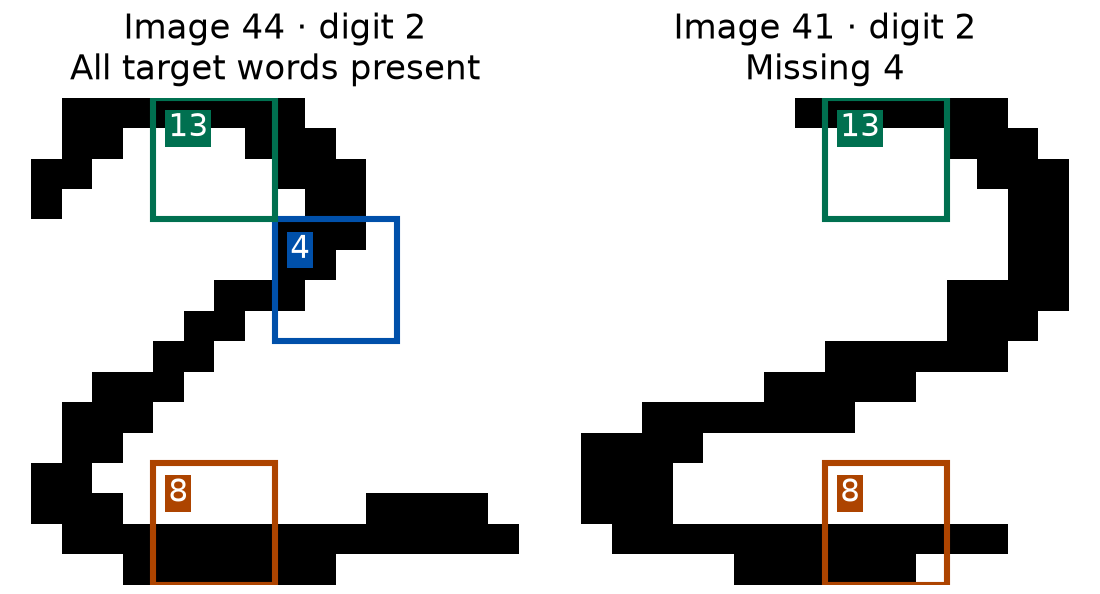
\includegraphics[width=\columnwidth]{figures/semeion-source-contrast.png}
\caption{Hai ảnh nguồn cùng nhãn chữ số 2 ở ngưỡng 5\%. Các ô vuông đánh dấu
patch được gán vào từ thị giác tương ứng. Ảnh 44 chứa đủ ba từ. Ảnh 41 thiếu
từ 4 theo ngưỡng khoảng cách của bộ mã hóa.}
\label{fig:semeion-contrast}
\end{figure}

Hình~\ref{fig:semeion-contrast} dùng tọa độ và pixel đã đối chiếu với dữ liệu
nguồn. Để kiểm tra độ nhạy, nhóm thay đổi kích thước từ điển $K$ và giữ nguyên
seed, cách cắt patch, số pixel nét tối thiểu, số vòng k-means và ngưỡng khoảng
cách. Trong mỗi lần đổi minsup, giao dịch và từ điển được giữ cố định.
Bảng~\ref{tab:semeion-sensitivity} ghi số itemset tìm được trên cùng 1.593 ảnh.

\begin{table}[t]
\centering
\caption{Độ nhạy của số itemset khi đổi kích thước từ điển và minsup.}
\label{tab:semeion-sensitivity}
\begin{tabular}{r r r r r r r}
\hline
$K$ & Ảnh rỗng & 20\% & 10\% & 6\% & 5,5\% & 5\% \\
\hline
16 & 99 & 4 & 12 & 19 & 21 & 25 \\
24 & 11 & 6 & 18 & 35 & 43 & 46 \\
32 & 2 & 5 & 24 & 45 & 52 & 63 \\
\hline
\end{tabular}
\end{table}

Với $K=24$, từ 13 và cặp \{8,13\} có mặt ở cả năm ngưỡng. Bộ ba
\{4,8,13\} có support 90, đủ ngưỡng 5,5\% (88 ảnh) và thấp hơn ngưỡng
6\% (96 ảnh). Khi tăng $K$ từ 16 lên 32, độ rộng trung bình tăng từ 2,27
lên 4,31 từ/ảnh và số ảnh rỗng giảm. Tại 20\%, số mẫu lớn nhất nằm ở
$K=24$. Mỗi từ điển được khớp lại nên cùng một ID có thể chỉ hai nét khác
nhau. Một nét ngang phổ biến trong nhiều nhãn có thể phản ánh cách viết và
cách đặt lưới trên ảnh nhị phân 16$\times$16. Cách chọn ví dụ cùng nhãn giúp
kiểm tra kết quả cục bộ. Tần suất thu được mô tả tập ảnh Semeion và từ điển
được học trên tập này.
